\documentclass[10pt,letter]{article}

\usepackage{graphicx}
\usepackage{url}
%\usepackage{hyperref}
\usepackage{enumerate}
\usepackage{verbatim}
\usepackage{times}
\usepackage{mdframed}

% ***** Margins ************
\oddsidemargin 0.12 in
\evensidemargin 0.12 in
\textwidth 6.5in
\textheight 8.2in
\marginparwidth 0pt
\hoffset -0.1in
\voffset -0.3in
% *********************************


% Title Page
\title{PFMFind Manual\\\textsf{\small Version 0.5}}
\author{Aleksandar Stojmirovi\'c}

\begin{document}
\maketitle
\tableofcontents

% \begin{abstract}
% \end{abstract}
\newpage

\section{Overview}
Protein Fragment Motif Finder (PFMFind) is a system written mostly in Python enabling discovery of relationships between short fragments of protein sequences using similarity search. It supports queries based on score matrices and PSSMs obtained through an iterative procedure similar to PSI-BLAST.

PFMFind system consists of three major components: a PFMFind GUI (graphical user interface) client, a search engine for fast similarity search of datasets of short peptide fragments called FSIndex and a relational database (Figure \ref{fig:PFMFind_struct}). PFMFind client takes user input, and communicates with FSIndex and the database through its components. It passes search parameters in batches to FSIndex and receives the results of searches that are then stored in the database. It also retrieves the results from the database and displays them, together with available annotations, to the user. The annotations are stored in a separate BioSQL schema in the database.

PFMFind components communicate using the standard TCP/IP socket interface and can therefore be located on different machines. Since PFMFind is highly modular, the GUI client can be replaced by a Python script for non-interactive use.

\begin{figure}[!tpb]
\centerline{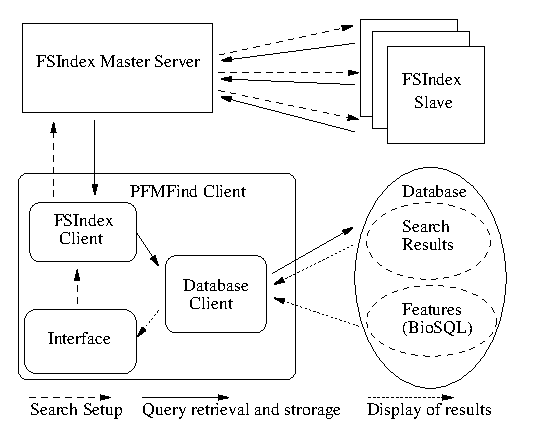
\includegraphics{PFMFind_struct.eps}}
\caption{Structure of PFMFind system.}\label{fig:PFMFind_struct}
\end{figure}

\section{Installation}

Each machine that runs the PFMFind client or FSIndex requires to have installed the PFMFind Python module and its prerequisites. A machine running the database needs to be have PostgreSQL installed. Here, we only describe installation of the Python module; for PostgreSQL-related instruction please refer to the appropriate PostgreSQL manual (\url{http://www.postgresql.org/docs/}).

\subsection{Prerequisites}
PFMFind requires Python2 (ideally version 2.7) with Tkinter. Before installing PFMFind you also need to download and install the following Python modules (the versions used for testing are indicated in square brackets):

\begin{itemize}
\item Numpy (\url{http://www.numpy.org/}) [1.6.2]
\item Scipy (\url{http://www.scipy.org/}) [0.11]
\item Biopython (\url{http://www.biopython.org/}) [1.58]
\item Pmw megawidgets toolkit (\url{http://pmw.sourceforge.net/}) [1.3.3]
\item psycopg2\footnote{It may be possible to replace psycopg2 with another PostgreSQL adapter.} (\url{http://initd.org/psycopg/}) [2.4.5]
\end{itemize}

(refer to the individual packages for the instructions on how to do so):

\subsection{Installing on UNIX platforms}

PFMFind is installed in the standard distutils way (see \url{http://docs.python.org/inst/inst.html}): Extract the source distribution, go to the top distribution directory and type
\begin{verbatim}
$ python setup.py install
\end{verbatim}
Please read the `Installing Python Modules' page (\url{http://docs.python.org/inst/inst.html}) for
customisation options. Note that you need a C compiler (such as gcc) to build the C extensions included in PFMFind.

\subsection{Other platforms}

Version 0.5 is currently not supported for platforms other than UNIX. You will need to build the entire package yourself (including C extensions) and install it as appropriate for your case.

\section{Database Setup}

\subsection{Quick guide}

\begin{enumerate}
\item Download the NCBI Taxonomy database from \url{ftp://ftp.ncbi.nih.gov/pub/taxonomy/} (this can be skipped and the taxonomy downloaded automatically by the {\it PFMFsetupdb.py} script.
\item Download the appropriate Uniprot, Uniref and Interpro files:
\begin{itemize}
\item UniprotKB files from \url{http://www.uniprot.org/downloads} in text (.dat) format;
\item Uniref files from \url{http://www.uniprot.org/downloads} in XML format;
\item Interpro file \texttt{protein2ipr.dat} from \url{http://www.ebi.ac.uk/interpro/download.html}.
\end{itemize}
\item Prepare the configuration file (see Subsection \ref{sec:dbconfig} below).
\item Run the {\it PFMFsetupdb.py} script (for example with configuration file \texttt{ dbsetup.xml}):
\begin{verbatim}
$ PFMFsetupdb.py dbsetup.xml
\end{verbatim}
\item Wait until the database is filled. If you have several configuration files associated with different steps, repeat the step 4. as needed.
\end{enumerate}

\subsection{PFMFsetupdb.py script}

The {\it PFMFsetupdb.py} script creates and loads the sequence database schema in the following sequence:
\begin{enumerate}
\item Creating a database schema and BioSQL tables;
\item Loading NCBI taxonomy information;
\item Loading Uniprot sequences and annotations;
\item Loading Uniref cluster information;
\item Loading Interpro domain informations.
\end{enumerate}
Depending on the configuration file, each step can be done separately or all together. The sequence however should be preserved except that steps 4. and 5. may be interchanged (or even totally omitted if only sequence/Uniprot data is required).



\begin{figure}[h!]
\begin{mdframed}
{\small
\begin{verbatim}

<?xml version="1.0" encoding="UTF-8"?>
<!DOCTYPE PFMF_db_setup SYSTEM "PFMFdb.dtd">
<PFMF_db_setup>
  <Database driver="psycopg" user="aleksand" db="PFMFind"/>
  <Schema name="SwissProt02082005" create="1"/>
  <Sql_scripts sql_start="biosqldb-pg-nocnstr.sql"
      sql_end="biosqldb-pg-cnstr.sql"/>
  <Taxonomy copy="1">
  <Taxon_dir>/home/aleksand/data/bio/taxon_tables</Taxon_dir>
  </Taxonomy>
  <Uniprot_file namespace="SwissProt">uniprot_sprot.dat</Uniprot_file>
  <Uniref_file namespace="SwissProt">uniref50.xml</Uniref_file>
  <InterPro_file namespace="SwissProt">protein2interpro.dat</InterPro_file>
</PFMF_db_setup>
\end{verbatim}
}
\caption{A sample full {\it PFMFsetupdb.py} configuration file (XML format)}\label{fig:config}
\end{mdframed}
\end{figure}

\subsection{Configuration file}\label{sec:dbconfig}

Figure \ref{fig:config} shows a sample configuration file. All configuration tags are under \texttt{ PFMF\_db\_setup} tag and the specification is given in the file {\it PFMFdb.dtd} located in the \verb|data/setup_config| directory of the PFMFind distribution. Hence, each configuration file can be checked for validity before being passed to {\it PFMFsetupdb.py}. Below is the description of each element and its attributes.


\subsubsection*{\texttt{ <Database>}}

This is a mandatory element that is empty and that must start the configuration options. It has six possible attributes:
\begin{enumerate}[(i)]
\item \texttt{ driver} -- mandatory: the PostgreSQL Python driver, usually {\it psycopg2} but others may work as well;
\item \texttt{ db} -- mandatory: the name of the PostgreSQL database to connect;
\item \texttt{ user} -- optional: database user name;
\item \texttt{ password} -- optional: database password;
\item \texttt{ host} -- optional: the host the database is running on (if left out, the localhost is assumed);
\item \texttt{ port} -- optional: the port on the host the database is listening to.
\end{enumerate}

\subsubsection*{\texttt{ <Schema>}}

An optional empty element (the default PostgreSQL schema is used if omitted) describing the schema that will contain the dataset and annotations. Two attributes:
\begin{enumerate}[(i)]
\item \texttt{ name} -- mandatory: the name of the schema;
\item \texttt{ create} -- optional: whether to create the schema, should be 1 if yes and 0 if the schema already exists. The default is 0.
\end{enumerate}

\subsubsection*{\texttt{ <Sql\_dir>}}

An optional element whose value is the path to the SQL scripts specified by the \texttt{ <Sql\_scripts>} element described below. The default is the current working directory.

\subsubsection*{\texttt{ <Sql\_scripts>}}

An optional element indicating the SQL scripts to be run to create the required tables. One script (attribute \texttt{ sql\_start}) is run at the beginning and the other (attribute \texttt{ sql\_end}) at the end of the run of {\it PFMFsetupdb.py}. If the tag is omitted, the default scripts are run. To skip a default script (for example, if the tables are already created), set its corresponding attribute to empty string.

\subsubsection*{\texttt{ <Taxonomy>}}

Optional element with one optional attribute (\texttt{ copy}). If specified, it must include the element \texttt{ <Taxon\_dir>}, which indicates the storage directory for the taxon data from NCBI. The \texttt{ copy} attribute can be set to 0 (default), 1 or 2. If it is 2, only the tab-separated tables will be loaded into database (this can be used to reuse the tables from several PostgreSQL schemas); if it is 1 the tables will in addition be created from the NCBI taxon data; if it is 0 the taxon data will be downloaded from the NCBI ftp site.

\subsubsection*{\texttt{ <Uniprot\_file>}, \texttt{ <Uniref\_file>}, \texttt{ <InterPro\_file>}}

These three tags describe the path to files containing the Uniprot, Uniref and InterPro data, respectively. Each can be repeated as many times as necessary (or omitted). The loaders for Uniref and InterPro consider only the annotations for those (Uniprot) sequences that were stored before -- hence, the order of tags is important. All three have the same attributes: \texttt{namespace} (mandatory, dataset identifier), \texttt{sql\_start} and \texttt{sql\_end} (optional SQL scripts to run before and after loading the data).

\section{Index Setup}

Indexes should be setup once the database is loaded using the script {\it PFMFsetupix.py}. The configuration is once again through an XML file (Figure \ref{fig:ixconfig}).

\begin{figure}[h!]
\begin{mdframed}
{\small
\begin{verbatim}

<?xml version="1.0" encoding="UTF-8"?>
<!DOCTYPE PFMF_index_setup SYSTEM "PFMFix.dtd">
<PFMF_index_setup>
  <Database driver="psycopg" host="130.195.61.38" port="5432"
            user="aleksander" password="aleksander" db="PFMFind"/>
  <Index_dir>/home/aleksander/data/uniprot-3.5/FSindex</Index_dir>
  <Dataset name="sprot" schema="PFMFind02" namespace="SwissProt"
           max_residues="80000000">
    <Index length="10">
      <Partition>STAN#ILVM#KRDEQ#WFYH#GPC</Partition>
    </Index>
    <Index length="12">
      <Partition>STAN#ILVM#KRDEQ#WFYHGPC</Partition>
    </Index>
  </Dataset>
</PFMF_index_setup>
\end{verbatim}
\caption{A sample full {\it PFMFsetupix.py} configuration file (XML format)}\label{fig:ixconfig}
}
\end{mdframed}
\end{figure}

\subsection{Configuration file}\label{sec:ixconfig}

The index configuration file is very similar to the database configuration file described above. All tags are under the \texttt{ <PFMF\_index\_setup>} tag and the specification is given in the file {\it PFMFix.dtd} located in the \verb|data\setup_config| directory of the PFMFind distribution. Below is the description of each element and its attributes.

\subsubsection*{\texttt{ <Database>}}

These are database connection details. Same as for database setup described in Section \ref{sec:dbconfig} above.

\subsubsection*{\texttt{<Index\_dir>}}

A mandatory element whose value is the path where the files containing sequences in FASTA format as well as the indexes are to be placed.

\subsubsection*{\texttt{<Dataset>}}

An element containing details about each dataset to be indexed. There can be multiple \texttt{<Dataset>} elements, each specifying multiple indexes.

It has four possible attributes:
\begin{enumerate}[(i)]
\item \texttt{name} -- mandatory: the dataset identifier used as a prefix for all files related to this dataset;
\item \texttt{schema} -- optional: the schema containing the dataset. If omitted, the setup script attempts to use the schemas from the default PostgreSQL path.
\item \texttt{namespace} -- optional: the namespace associated with the dataset (each schema can contain multiple dataset, each identified using the namespace identifier). If omitted, all sequences from the schema are retrieved.
\item \texttt{max\_residues} -- optional: the maximum number of residues a single sequence file can contain. If the dataset contains more than that number of residues, multiple files and indexes will be created\footnote{Each part will probably contain slightly more residues because the full sequences are not broken up.}. These parts can then be loaded by slave index servers and the whole search distributed by a master server.
\end{enumerate}

Each \texttt{<Dataset>} can contain one or more \texttt{<Index>} elements, whose only (mandatory) element is \texttt{length}, giving the fragment length to be used to create the index. In turn, each \texttt{<Index>} element contains one or more \texttt{<Partition>} elements, having no attributes and containing a string specifying the amino acid alphabet partitions.

Alphabet partitions are separated by \texttt{\#} (e.g. \texttt{STAN\#ILVM\#KRDEQ\#WFYH\#GPC}) and each \texttt{<Partition>} element specifies an alphabet partition for a single position in the fragment (up to the fragment length). If there are fewer \texttt{<Partition>} elements than the specified fragment length, the last \texttt{<Partition>} element is used for all remaining positions. Hence, in order to have the same alphabet partitions at all positions, it is sufficient to specify a single \texttt{<Partition>} element.

\section{Running FSIndex search servers}

There are two types of an FSIndex server: a slave, which actually loads an index and conducts searches and a master, which distributes and collects searches. They communicate between themselves and with clients using TCP/IP sockets.

The master/slave configuration can be used in the case where indexes are located on different machines, even running different operating systems. If there is only one server, it runs under the slave configuration. This means that each slave can be queried individually and also that a more complicated tree-like structure, where inner nodes are master servers and leaves are slaves, can be constructed if needed.

Two scripts can be used to run an FSIndex server: \textit{FSsearchd.py}, and \textit{FSsearchc.py}. \textit{FSsearchd.py} runs as a UNIX daemon, while \textit{FSsearchc.py} is a regular script for all platforms. Their arguments and options are very similar and are described in detail only for \textit{FSsearchd.py}.

\subsection{FSsearchd.py daemon}\label{sec:FSdaemon}

\textit{FSsearchd.py} script starts an FSIndex server as a UNIX daemon. Unlike the other script, the master slave can be passed an option to control its slaves, in which case it starts the slaves using ssh\footnote{Note that the current version assumes that the ssh login is using public key without a password.} on startup and shut them down when it terminates.

\subsubsection{Starting}

\textit{FSsearchd.py} daemon is started from the command line:
\begin{verbatim}
$ FSsearchd.py [-c] serverid port workpath indexfile [pythonpath]
\end{verbatim}
where
\begin{itemize}
\item \texttt{serverid} is a string identifier of a particular index (or set of indexes) being loaded;
\item \texttt{port} is the port the daemon should be listening;
\item \texttt{workpath} is the path to the directory where log files are to written;
\item \texttt{indexfile} is the path to the index file. If the file ends with \texttt{.cfg}, it is assumed to be a configuration file for the slaves;
\item \texttt{pythonpath} (optional) is appended to the system's python path. This may help in the case that the proper path to Python modules required by \textit{FSsearchd.py} is not set as an environment variable.
\end{itemize}

The option \texttt{-c} (long version \texttt{--control-slaves}) can be used to instruct a master server to attempt to start and terminate its slaves using ssh. If this option is omitted, the master will only attempt to contact each slave and, if any one is unavailable, shut itself down. In that case the slaves must be started separately.

A master's configuration file is a text file where each line gives parameters for a slave server to be started. The format of each line is:
\begin{verbatim}
host port workpath indexfile [pythonpath [binpath]]
\end{verbatim}
where the fields are separated by spaces. The fields \texttt{port}, \texttt{workpath}, \texttt{indexfile} and \texttt{pythonpath} are used directly to start the slave server (see above for full description). The field \texttt{host} specifies the address of the machine the slave is running on. The optional \texttt{binpath} gives the path to the \textit{FSsearchd.py} executable on the host the slave should run on. Only \texttt{host} and \texttt{port} fields are used if \texttt{-c} is not set.

Each server produces two files: a log file and a pid file. The log file receives detailed messages about the running of the server while the pid file contains the UNIX process id of the daemon, the name of the host it is running on, as well as the command line used to start it. The name of the log file is generated from the \texttt{serverid} passed as a command line argument. If a master is starting its slaves, it passes its own \texttt{serverid} to them, concatenated with the number of the slave. For example, a master server passed \texttt{TEST2} as \texttt{serverid} will produce the logfile named \texttt{FSsearchd\_TEST2.log} and its second slave will produce \texttt{FSsearchd\_TEST2\_s01.log}.

\subsubsection{Terminating}

Since \textit{FSsearchd.py} is a daemon and hence not connected to any terminal, the best way to terminate it is to send it a SIGTERM signal. To do so, find out (from a pid file or the output of \textit{ps}) its process id (\texttt{pid} and type
\begin{verbatim}
$ kill pid
\end{verbatim}
This is a clean way to shutdown an FSIndex server since the logs are written and any pending requests are handled before shutdown.

\subsection{FSsearchc.py script}\label{sec:FSscript}

\textit{FSsearchc.py} script runs an FSIndex server from the command line, printing log to the standard output. It should run on all platforms and is started by
\begin{verbatim}
$ FSsearchc.py port indexfile
\end{verbatim}
where the parameters are as described in Subsection \ref{sec:FSdaemon} above. It can be stopped by killing the server process.

\section{Running GUI client}

\subsection{Starting}

The GUI client can be started (on both UNIX and Windows) from the command line using the \textit{PFMFind.pyw} script:
\begin{verbatim}
$ PFMFind.pyw [--console] [config_file]
\end{verbatim}

The client will contain a Python console if the option \texttt{--console} is set. The \texttt{config\_file} optional argument is the path to an XML file containing the information about the database and the index to be connected. This file can also be specified from the GUI.

\subsection{GUI functionality}

TO DO.

\section{Beyond GUI}

\subsection{Search matrix plugins}

Writing plugins is quite easy (as far as the interface is concerned). A plugin is a python module that defines two global variables, \texttt{iteration} and \texttt{arg\_list} as well as two functions: \texttt{get\_matrix} and \texttt{print\_info} (optional).

\begin{itemize}
\item The variable \texttt{iteration} is a constant being either \texttt{True} or \texttt{False}. If it is set to \texttt{True}, the plugin can be used in the second or subsequent iterations, otherwise it is only used for the first iteration.

\item The variable \texttt{arg\_list} is a list specifying the arguments of the functions \texttt{get\_matrix} and \texttt{print\_info}. Its elements are triplets of the form \texttt{(Name, Type, Default\_value)}, where name is a string identifying the variable (it is displayed on the GUI), the type is either a string or a list of strings. In the former case the GUI sets up a Pmw EntryField widget whose value type is given by the string (Please refer to Pmw documentation). In the latter case, a Pmw OptionMenu is setup with options being the members of lists. In both cases the given default value is preselected.

\item The function \texttt{get\_matrix} does all real work for matrix construction. It receives as a first argument a hit list from the previous iteration followed by any other arguments as they appear in the \texttt{arg\_list}. It must return a 3-tuple of the form \texttt{(M, matrix\_type, ctype)}, where \texttt{M} is a Biopython-style score matrix or PSSM, \texttt{matrix\_type} is 0 if the matrix is a score matrix and 1 if it is a PSSM, while \texttt{ctype} should be set to 0 if the matrix contains similarity scores (the other values are for distance based matrices ...).

\item The (optional) function \texttt{print\_info} takes the same arguments as \texttt{get\_matrix} and returns a printable string showing (in a human-readable way) the matrix produced by \texttt{get\_matrix}.

\end{itemize}

\end{document}
